\section{Integration Test Plan Document}

\begin{frame}
	\frametitle{Entry Criteria}
	\begin{itemize}
		\item RASD and DD documents are completely composed
		\item Development goes forward along with their unit testing
		\item Every component has at least 90\% of its functionalities completed
		\item The integration process starts at the achievement of the following percentages of development:
		\begin{itemize}
			\item 100\% of the Database and Availability Helper components
			\item at least 80\% of the Controller components
			\item at least 50\% for the client applications
		\end{itemize}
	\end{itemize}
\end{frame}

\begin{frame}
	\frametitle{Integration testing strategy}
	\qquad \textbf{Bottom-up approach}
	\begin{itemize}
		\item Components integrated from the most independent to the less one
		\item Avoiding useless stubs
		\item Creation of an integrated subsystem
		\item Allowing developers to perform integration testing earlier in the development process
		\item Parallelism and efficiency are maximized
	\end{itemize}
\end{frame}

\begin{frame}
	\frametitle{Components}
	\vspace*{-0.5cm}
	\begin{figure}[H]
		\centering
		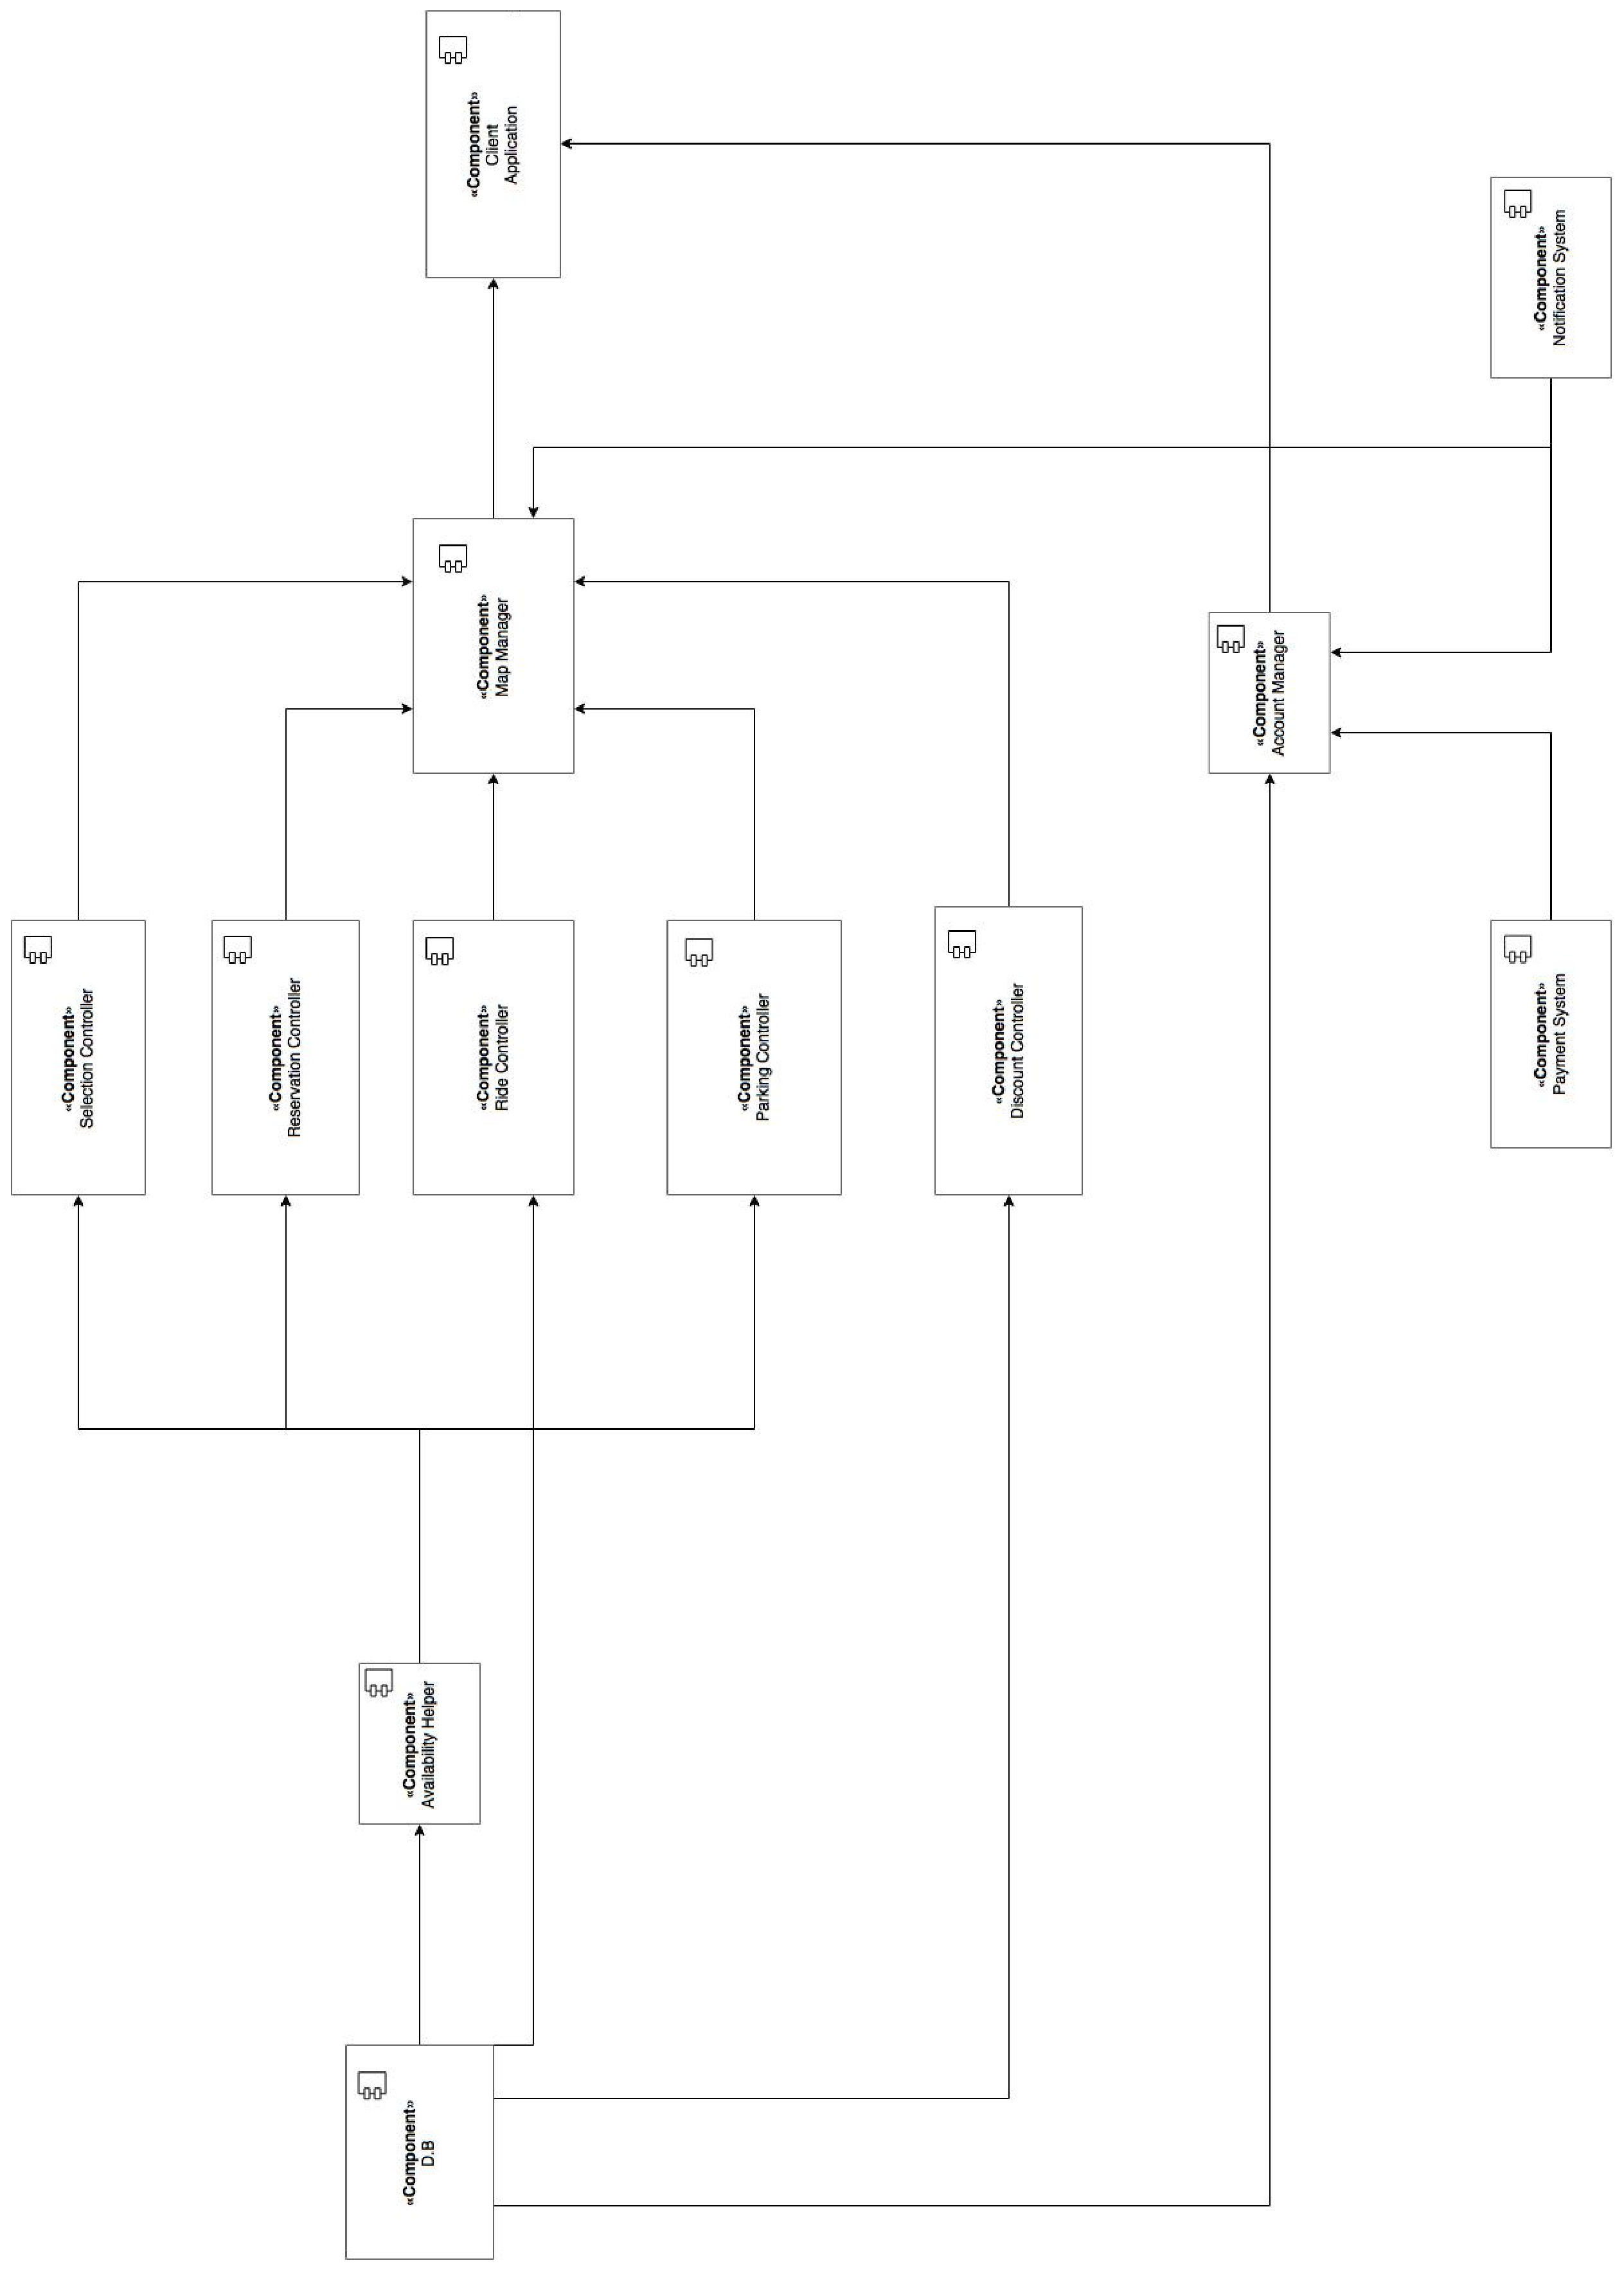
\includegraphics[height=10.5cm,keepaspectratio,angle=270]{figures/components_controller.eps}
		\label{fig:components_controller}
	\end{figure}
\end{frame}

\begin{frame}
	\frametitle{Integration Test Cases}
	\begin{table}[H]
		\centering
		\begin{tabular*}{\textwidth}{p{4.4cm} @{\extracolsep{0.5cm}} p{8.5cm}}
			\hline
			\textbf{Test case identifier} & I5T2 \\
			\hline
			\textbf{Test item(s)} & Reservation Controller \(\rightarrow\) Map Manager \\
			\hline
			\textbf{Input specification} & Post a ReservationController request \\
			\hline
			\textbf{Output specification} & Check if the request is correctly routed \\
			\hline
			\textbf{Environmental needs} & I1, I2, I3 succeeded \\
			\hline
		\end{tabular*}
	\end{table}
	\begin{table}[H]
		\centering
		\begin{tabular*}{\textwidth}{|p{4.0cm}|p{7.18cm}|}
			\hline	
			\multicolumn{2}{|c|}{placeReservation(car) returns response} \\
			\hline
			\textit{Input} & \textit{Effect} \\
			\hline
			A valid car & ReservationController will invoke AvailabilityHelper.changeTagRequest() and get the response R. R is then returned. \\
			\hline
			A null or invalid car & A NullCarException or InvalidCarException is generated. \\
			\hline
		\end{tabular*}
	\end{table}
\end{frame}

\begin{frame}
	\frametitle{Program Stubs}
	\begin{itemize}

		\item Reduced number of drivers is required to perform necessary method invocations
		\begin{itemize}
			\item \emph{AvailabilityHelper driver}: invokes the methods exposed by the component AvailabilityHelper in order to test its interaction with the database management system
			\item \emph{Controllers driver}: invokes the methods exposed by the Controllers (acting like MapManager) in order to test its interaction with each other
		\end{itemize}
		\item Only one stub acting like the client to fulfill the request/response protocol during client/system interaction
	\end{itemize}
\end{frame}